\section{Quicksort}
\label{sec:safe_the_best_for_last}


\begin{frame}
	\frametitle{Quicksort}
	\framesubtitle{XKCD Ineffective Sorts: \url{https://xkcd.com/1185/}}
	\begin{center}
		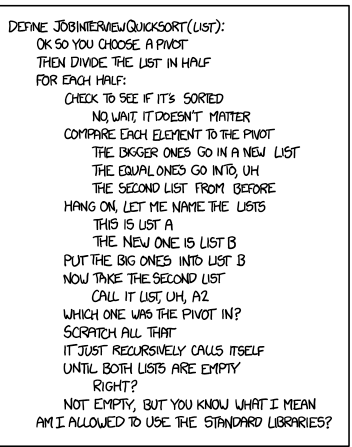
\includegraphics[width=0.4\textwidth]{figures/quicksort.png}\\
	\end{center}
\end{frame}

\begin{frame}
	\frametitle{Quicksort}
	\begin{block}{Quicksort}
		A recursive sorting algorithm.\\
		\pause
		It splits the list into two, sorts each half, then combines the results.
	\end{block}	
	\pause
	\begin{alertblock}{Wait...}
		That sounds exactly like mergesort!?
	\end{alertblock}	
	\pause
	\begin{exampleblock}{Yes}
		But this is often even better :)
	\end{exampleblock}	
\end{frame}

\begin{frame}
	\frametitle{The idea}
	\begin{overlayarea}{\textwidth}{\textheight}
		\begin{columns}
			\column{0.705\textwidth}
			The algorithm:
		\begin{algorithmic}
			\Function{Quicksort}{xs}
			\If{len(xs) $< 2$}	
			\State \Return xs
			\EndIf
			\pause
			\State pivot $\gets$ some element from xs
			\State left $\gets$ everything smaller than pivot
			\State right $\gets$ everything larger than pivot
			\State leftHalf $\gets$ \Call{Quicksort}{left}
			\State rightHalf $\gets$ \Call{Quicksort}{right}
			\pause
			\State \Return \alt<5->{leftHalf + pivot + rightHalf}{\dots}
			\EndFunction
		\end{algorithmic}
		
			\column{0.305\textwidth}
			\only<4>{
			\begin{questionblock}{What do we do here?}
				\begin{enumerate}[A.]
					\item Merge the left and right half.
					\item Return left + right
					\item Return left + pivot + right
					\item Return right + pivot + left
				\end{enumerate}
			\end{questionblock}
				}
			\only<6>{
				\begin{questionblock}{What I thought this was better?}
					What is the time complexity of this?\\
					Or rather, what does the worst case input look like?
			\end{questionblock}
				}
		\end{columns}
	\end{overlayarea}
\end{frame}

\begin{frame}
	\frametitle{It depends!}

	\begin{answerblock}{It depends!}
		Everything stands and falls by the choice of pivot.
	\end{answerblock}
	\pause
	\begin{questionblock}{The first element}
		What is the worst input if we always take the first element as the pivot?
		\begin{enumerate}[A.]
			\item A sorted list
			\item The reverse of a sorted list
			\item A list that has the first $n/2$ elements sorted ascendingly and the second $n/2$ elements sorted descendingly.
		\end{enumerate}
	\end{questionblock}
	\pause
	\begin{answerblock}{A sorted list}
	 This takes of only $1$ element every time, meaning we need $O(n^2)$ time.	
	\end{answerblock}
\end{frame}

\begin{frame}
	\frametitle{In practice}
	
		\begin{block}{Quick Sort in the real world}
			\begin{itemize}
				\item It is the most common sorting algorithm used.
				\item The implementations choose \textit{random} pivots.
					\pause
				\item Worst-case this is still $O(n^2)$ of course.
					\pause
				\item But with some fancy analysis (that we will not go into today, but maybe tomorrow ;)), we can show that
					this is $O(n \log n)$ in expectation (average case if you will).
					\pause
				\item In practice this often outperforms merge sort significantly, especially when we make it in-place.
			\end{itemize}
		\end{block}	
\end{frame}

\begin{frame}
	\frametitle{Let's do one example!}
	\begin{block}{But on the smartboard}
		Making this in Tikz is way too much effort ;)
	\end{block}		
\end{frame}

\begin{frame}
	\frametitle{Quicksort: pros and cons}
	\begin{block}{Quicksort}
			Recursively split the list in smaller and larger elements, sort and combine.
		\end{block}	
		\begin{exampleblock}{Pros}
			\begin{itemize}
				\item Great time complexity for average case $O(n\log n)$
				\item Simpler to implement (and faster in most cases) than merge sort.
				\item Argument based on authority: the whole world uses it.
			\end{itemize}
		\end{exampleblock}	
		\begin{alertblock}{Cons}
			\begin{itemize}
				\item Still $O(n^2)$ if we are unlucky in choosing pivots.
			\end{itemize}
		\end{alertblock}	
\end{frame}
